\chapter{Literature Review}

\section{Introduction}

A roster, sometimes referred to as a rota or schedule, is a list with dates (or shifts) with staff, such as employees or volunteers assigned to them, indicating what work will be done and when it will be done. It might also indicate when staff are unavailable, such as them being on leave. \cite{CollinsRoster}

Automatically assigning staff to a roster is a well-known problem in computing. As described by Ernst et al, it is highly challenging to 'determine optimal solutions that minimise costs, meet employee preferences, distribute shifts equitably among employees and satisfy all the workplace constraints.' \cite{ERNST20043}. As described, 'hard' constraints must be conformed to in order for the roster to be deemed valid. Such constraints might include: \cite{Chen2016}

\begin{itemize}
    \item Availability of staff - staff cannot be away or on leave
    \item Staff cannot carry out more than a certain number of consecutive shifts
    \item Staff cannot exceed maximum numbers of shifts, or fall under a given minimum
    \item Staff must be of the right sub-type, or meet criteria such as skill level or qualification
\end{itemize}

The efficiency of the outcome is determined not only by its validity, but also by how well it meets 'soft' constraints, such as regularity of shifts.

In general, software for tackling this problem exist to reduce the intrinsic difficulties and time overheads presented by manually rostering workforce, which was a role traditionally carried out continuously by secretarial staff, who would ensure that constraints where not violated as aforementioned, and would optimise the rota as much as possible for the sake of soft constraints to be best met. Today, most of this work is done by software, although occasionally conflicts must be resolved by a human. \cite{Maes1994AgentsTR}

Based on the project's aims and objectives, it is already established that an automated or semi-automated solution to automatically roster staff is unnecessary and beyond the scope of the application, as there are dedicated personnel responsible for ensuring that necessary gaps are filled, and volunteers add themselves to roles which they are qualified to fulfill at their own discretion. Nevertheless, having an understanding for this computational problem remains useful for the design and implementation of the project and is subsequently worth researching.

\section{The Nurse Scheduling Problem (NSP)}
The aforementioned problem of automatically finding the most optimal way to assign workers to shifts, with both hard constraints that must be met in order to be valid, and soft constraints that determine the optimality of the solution, is commonly referred to as the Nurse Scheduling Problem (henceforth NSP) and is considered by most sources to be of NP-hard (non-deterministic polynomial time) complexity. \cite{Tassopoulos2013} 

The reason behind nursing being the focus for this particular scheduling problem is that it is particularly challenging to roster for shifts that exist around the clock (healthcare institutions such as care-homes and hospitals work during the day and night), that require staff with varying required skill and competency levels for different types of work, whilst also ensuring that other soft constraints such as regularity and routine of schedules to benefit nurse wellbeing are met. \cite{Burke2004}

This has a strong parallel with the current challenges presented by the steam railway, where although there exists only one shift per day, vastly simplifying the problem, there is also a need for various volunteers with different skill levels and related constraints to be met.

The two most well-researched and documented solutions to this problem involve the usage of genetic algorithms, and simulated annealing (including derivative methods), although other implementations have been explored in detail.

\subsection{Genetic Algorithms (GA)}
Genetic algorithms (GA) are described by McCall as a heuristic search and optimisation technique originating in the 1960s that is modelled on Darwinian natural evolution, whereby a population of chromosomes - each a solution to a problem and a measurement of its effectiveness, called fitness. Those with the highest fitness are combined to produce new child chromosomes, and this process continues until criteria pertinent to the solution are met. \cite{MCCALL2005205}

Furthermore, random mutations have a possibility of occurring on each new generation, further modelling the real-world phenomenon of evolution and to diversify the population of chromosomes, as well as to increase the possibility of discovering the most optimal solution. \cite{AUGUSTINE2009}

\subsection{Simulated Annealing}
Baird describes simulated annealing as an optimisation algorithm that is used to find global optima in the presence of local optima. He explains that moves are randomly selected and always accepted if the current solution is improved as a result of that move. Should this not be the case, the move has a chance of being made anyway, with the probability determined based on the 'badness' of the move, which in turn is determined by the quantity in which the solution is made worse. \cite{Baird1998}

As written by Press et al, the name of this algorithm is derived from an analogy with its namesake in thermodynamics, in the way that 'liquids freeze and crystallize, or metals cool and anneal' and how when high temperature liquids are cooled slowly, 'atoms are often able to line themselves up and form a pure crystal that is completely ordered'. \cite{Press:1992:NRC:148286}

Ko et al explains that simulated annealing is an acceptable means of providing a good solution rather than the most optimal one, and that more accurate results can be obtained within shorter periods of time by using Cost Matrix-based simulated annealing (CSMA), a derivative method using a cost matrix for the transition rule. \cite{ko2013efficient}

\section{Prominent Rostering Solutions}
As scheduling software began to come into prominence in the 1980s as manual work tracking systems and spreadsheet-based solutions, digital software solutions specifically intended for the rostering of volunteer staff started to arise as a more efficient replacement. While countless solutions exist, and software specifically designed for paid members of staff could also be used for rotaing volunteers, three well-known solutions have been explored. The first of which, is a bespoke solution specifically designed for historic railways. The following two are generic solutions that are popular solutions for volunteer-based organisations.

\subsection{Heritage Operation Processing (HOPS)}
Heritage Operation Processing (HOPS) is a timetabling, rostering, and management solution designed specifically for railway operators by railway operators, designed to speed up and make more accurate time-consuming processes, including timetabling and rostering, and it began development in Gloucestershire Warwickshire Railway in August 2009. \cite{Hops1}

\begin{figure}[!ht]
    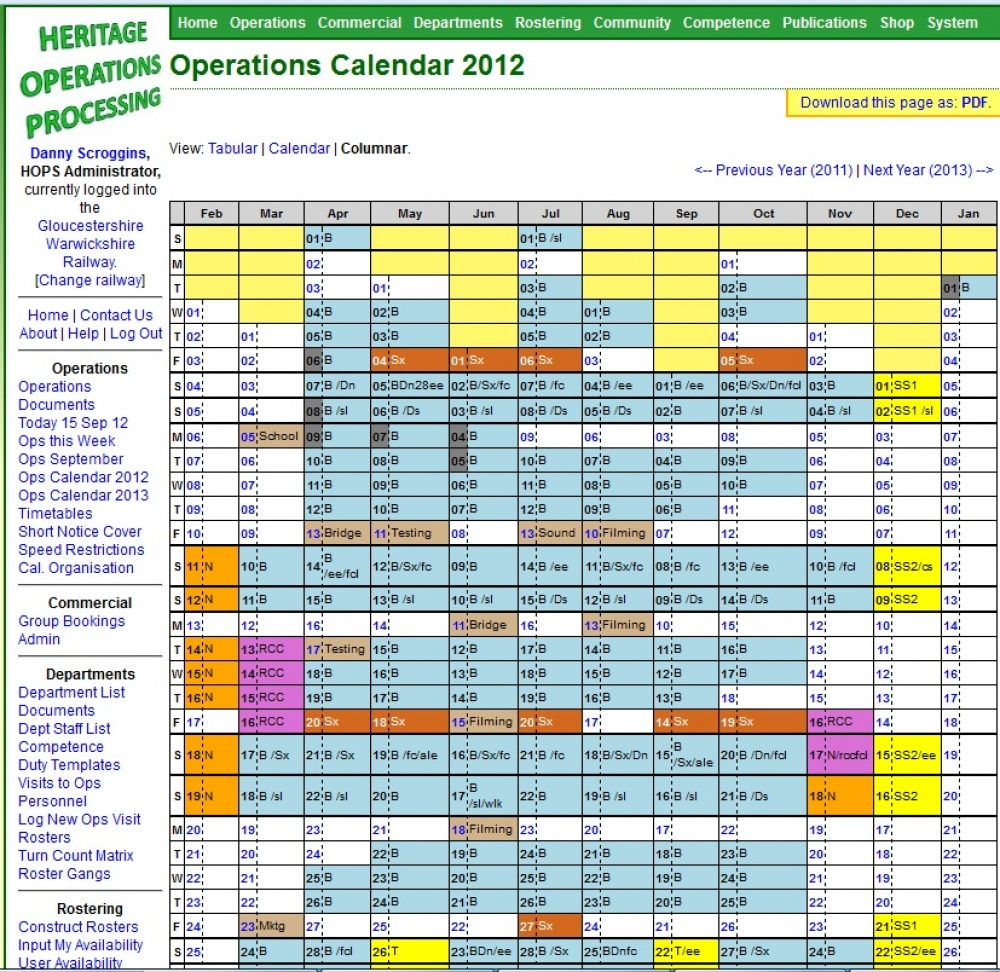
\includegraphics[width=\textwidth]{Figures/hops-operations}
    \caption{The Operations UI as displayed in HOPS.}
    \label{fig:hops} \cite{Hops3}
\end{figure}

The wealth of experience and domain knowledge displayed by the developers of HOPS in their product is clear, as not only does the product go above and beyond the requirements for this project, but it also offered a wealth of functionality, included fully automated rostering functions, but also discussion forums allowing for communication of users, invoicing and financial systems, and even the ability to order, track, and pay for commonly required equipment from HOPS themselves. This functionality appears to be fully customisable, and clients can opt out of functionality that they do not want. The vast majority of HOPS' functionality can be used free-of-charge. \cite{Hops1} \cite{Hops2}

\begin{figure}[!ht]
    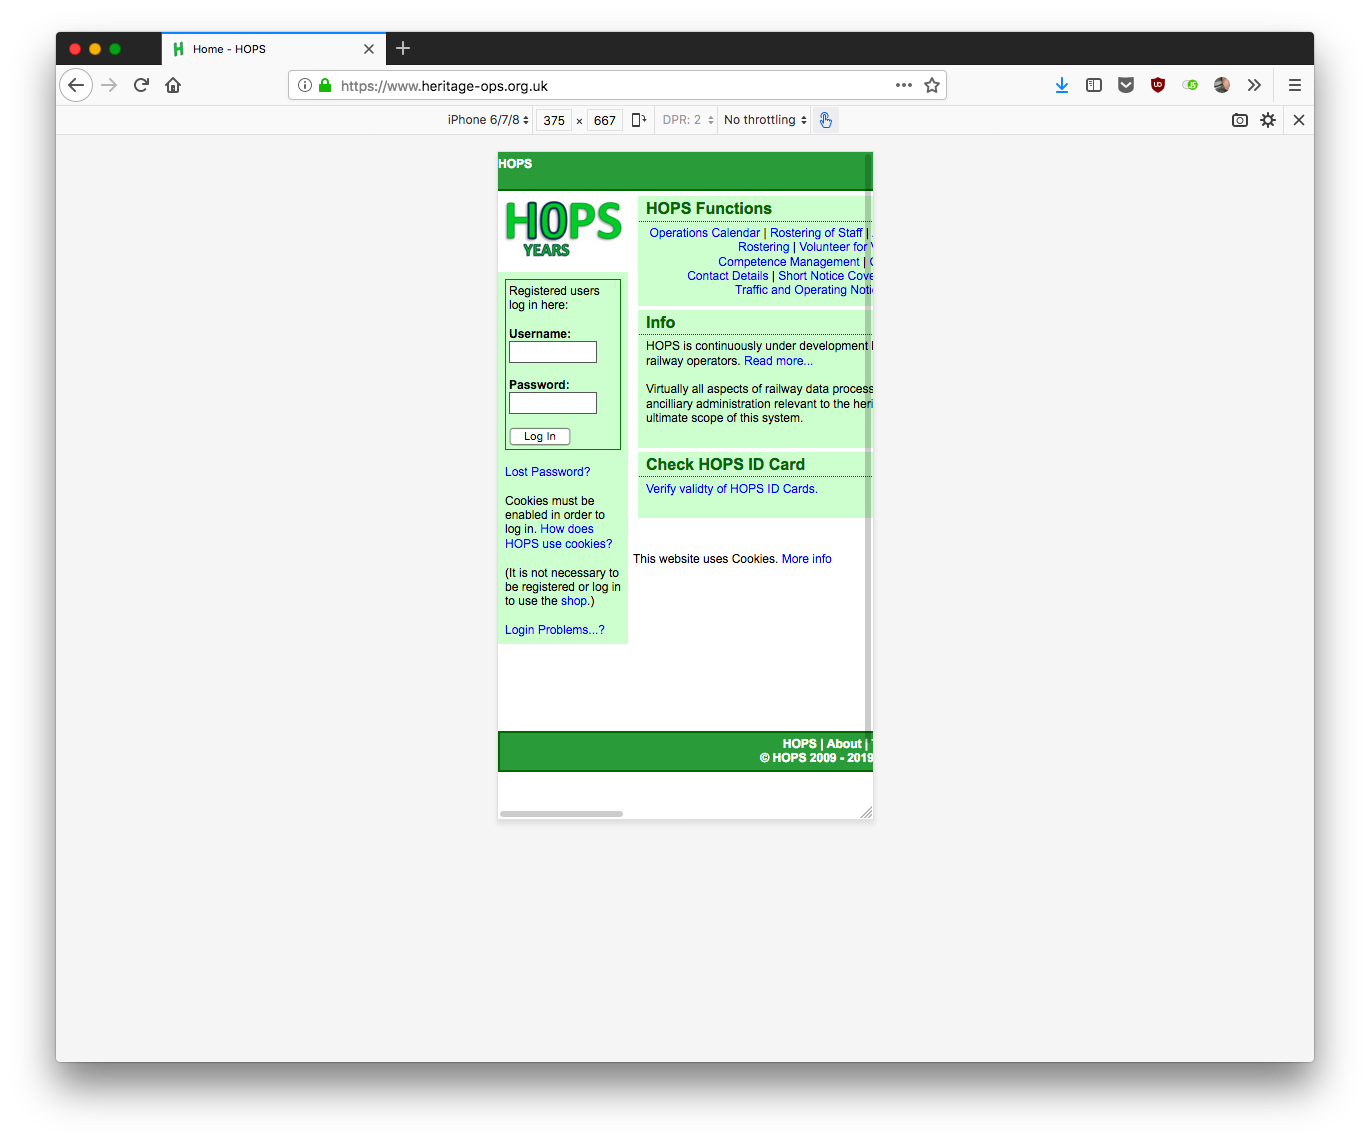
\includegraphics[width=\textwidth]{Figures/hops-unresponsive}
    \caption{HOPS interface is not responsive, as shown in Mozilla Firefox Responsive Design Mode.}
    \label{fig:hops2}
\end{figure}

While HOPS does fulfill the customers requirements almost in full, the interface is visibly complex and difficult to use. Oral conversations with the client revealed that they are well aware of HOPS, but the difficulty in using the interface is a put off for the majority of volunteers, and as a result they resort to using manual spreadsheet solutions as shown in Appendix \ref{Example Timetable}. In addition, HOPS is not responsive, and does not resize itself properly in order to operate in smaller viewports, such as that of a smartphone or tablet. This would require some redesign of the web application front-end and the inclusion of media queries in order to rectify. \cite{6976522}

\subsection{Three Rings}

Three Rings is an online volunteer management system that is entirely run by volunteers, and is at this time of writing used by prominent charities such as The Samaritans, Macmillan Cancer Support, and Citizens Advice. \cite{3r1} It was founded by Dan Q whilst volunteering for Aberystwyth Nightline in 2002, a student-run listening service that catered for the needs of students at Aberystwyth University. \cite{Q1} \cite{AberNL1} In addition, Three Rings has a flexible pricing system, whereby smaller charities and helplines are charged very little, as low as £40 a year, expanding to £600 for nationwide charities - the fee expected is derived from an organisation's annual turnover and volunteer count. \cite{3r4}

\begin{figure}[!ht]
    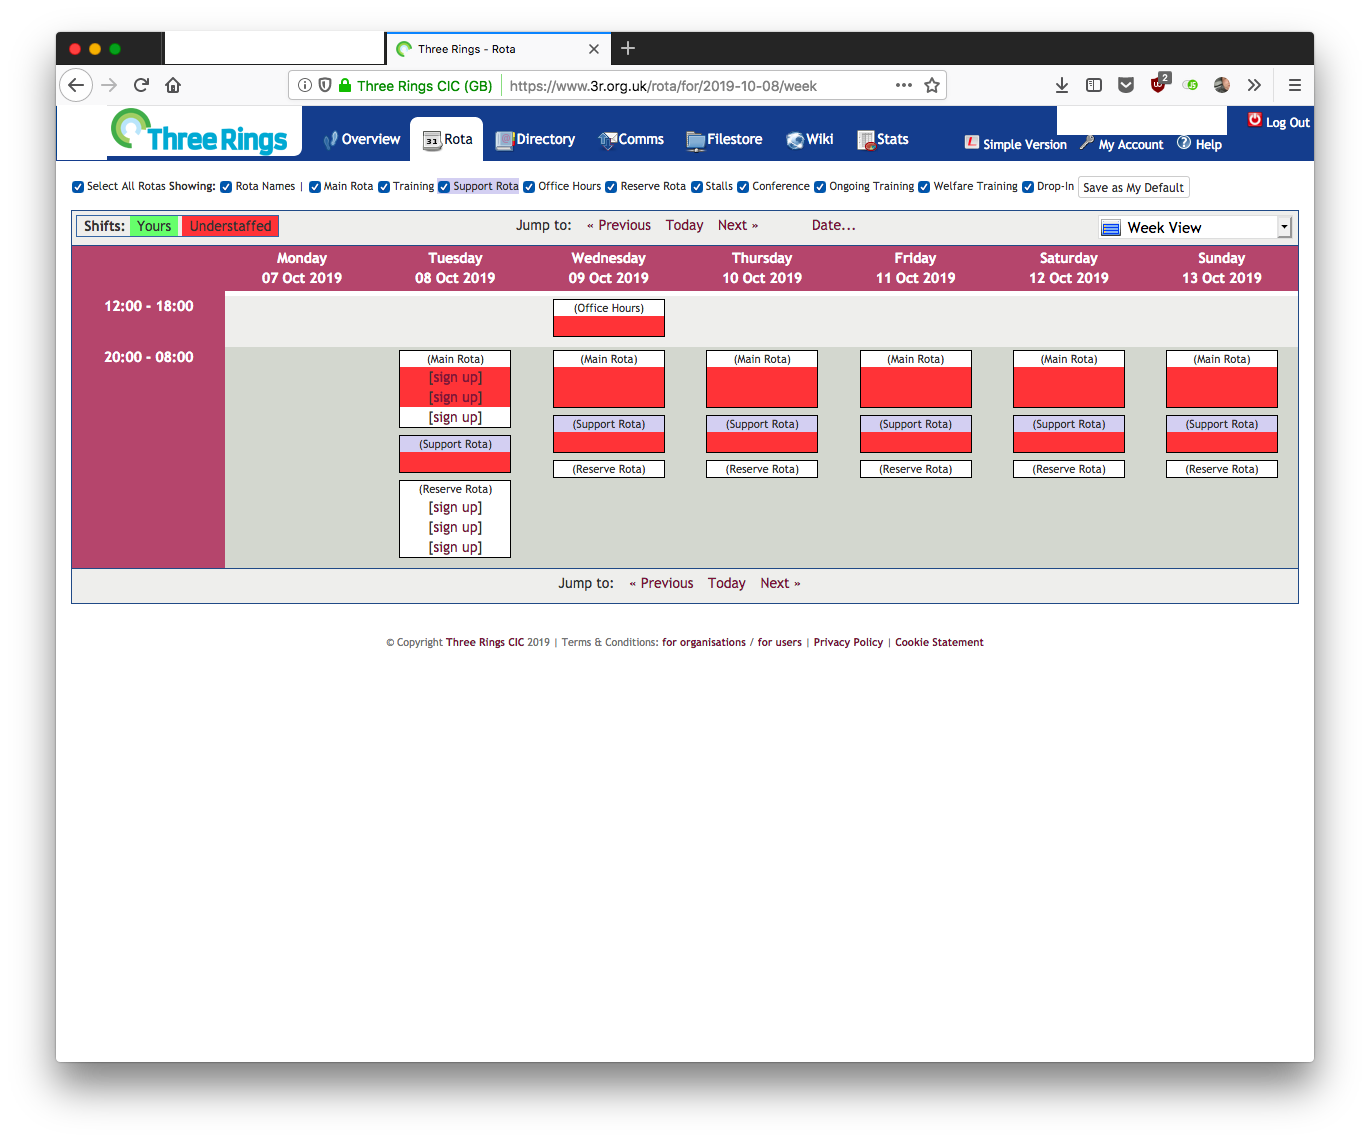
\includegraphics[width=\textwidth]{Figures/3r}
    \caption{Three Rings interface as seen on a desktop web browser, with confidential data redacted.}
    \label{fig:3r}
\end{figure}

Like HOPS, Three Rings is centred around rota functionality that allows for different kinds of shifts to be defined, and users can view and modify their own information. Resultingly, as the application is also designed and subsequently advertised as a mobile-friendly application, it can be easily utilised on a handheld device, and meets all the customer's requirements. Furthermore, the software includes complex stats reporting and an area for uploading and sharing files, as well as support for algorithmically populating vacant rosters with eligible volunteers. \cite{3r3} \cite{3r2}

Finally, Three Rings was recommended, alongside more rudimentary freeware solutions such as Google Calendar, by Voluntary Action Sheffield in a review of various volunteer shift and rota solutions, described as a 'low cost option with a large range of features.' \cite{SVC1}

\subsection{ABC Roster} 

ABC Roster is a proprietary freeware rostering application that is now used by a wide range of businesses and charitable organisations that prides itself on being easy to use, 'with a convenient and intuitive way of creating schedules quickly.' It appears to include all required functionality, such as availability management, the ability to email staff, as well as desirable bonus functionality such as the automated production of schedules and exportability. \cite{ABC1}

\begin{figure}[!ht]
    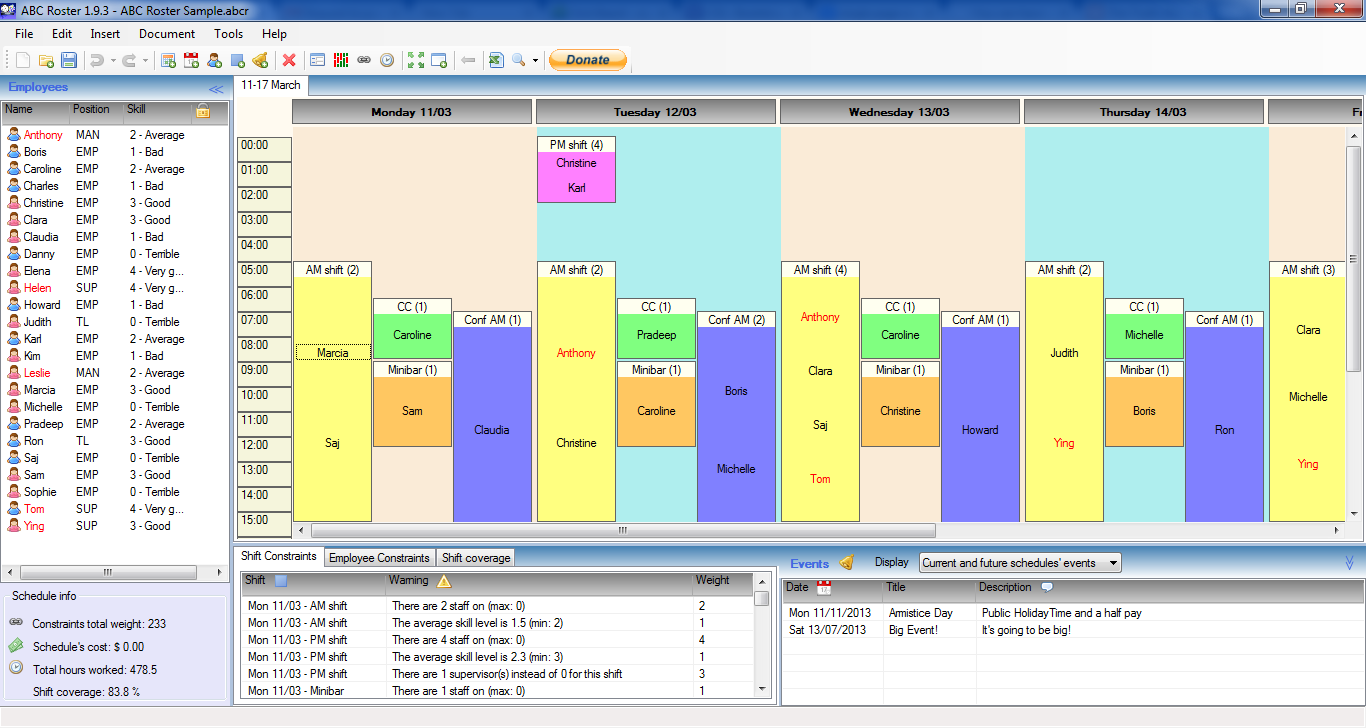
\includegraphics[width=\textwidth]{Figures/abcroster}
    \caption{ABC Roster interface, shown running on Microsoft Windows.}
    \label{fig:abc} \cite{ABC1}
\end{figure}

While a strong contender, with a wealth of functionality and sporting an interface that is straightforward to use, this is a desktop application for Windows, and is both not available for other platforms, such as macOS or GNU/Linux, and is not usable on mobile devices, as it is neither a mobile or web-based application. As the application needs to be able to run on the system requirements outlined on Appendix \ref{Operating Environment}, this is clearly an issue, beyond violating the requirements of a web-based application that can also be accessed on mobile.

In spite of this, there are things that can be taken away from ABC Roster and noted in the construction of a new solution. It's capability to define different roles with differing competencies is noteworthy, as well as the capacity to export rotas into printable form. \cite{ABC1} The software's documentation also provides a detailed insight into the workings of the algorithm responsible for automatically filling in rosters with staff - identifying constraints, weights, and penalties, with an algorithm in likeness to simulated annealing as explored previous:

\[ (3x - 2y) * 4w \]

Let x as the required number of employees; y as the actual number of employees, and w as the constraint weight. The penalty for satisfied constraints is zero. \cite{ABC2}

\section{Research Conclusion}
While as previously discussed, resolving the NST and implementing an automated rostering solution is beyond the scope of this project, it provides an important insight into the maturity of the computational problem, and importantly the solutions that exist to address said problem, including the software packages in which they are contained. This research is nevertheless a valuable pursuit, as with all agile software projects, there is nothing prohibiting this functionality to become desirable in future revisions, or even as a desired inclusion into an early deliverable. As stated by Ambler, 'project stakeholders have the right to define new requirements, change their minds about existing requirements, and even re-prioritise requirements as they see fit.' \cite{Ambler2}

The investigation of existing software solutions has provided a wealth of insight into shared functionality, what solutions do well, and some of their shortcomings that renders them inappropriate. It can be safely concluded from the research that a solution like Three Rings is very ideal for the task at hand, and subsequently this software project should look to emulate its offerings in some form, whilst incorporating domain specialism demonstrated by a product such as HOPS. In a nutshell, this research has provided valuable insight into what the ideal software solution looks like: responsive and easy to use, with a UI that is similar to the existing calendar / spreadsheet system, and specifically catered for the Corris Railway.

Should this research be continued or expanded upon, it would be ideal to explore even more examples of rostering software, including those used by major corporations and organisations that are not explicitly within the third sector. Furthermore, additional research into implementations of NST solutions is a good direction, so that should this be desired in a future revision of the software, it can be readily and promptly installed.